\section{Modelos Básicos de Sistemas de Recomendação}
\subsection{Filtragem Colaborativa \textit{Neighborhood-based}} A filtragem
colaborativa baseada em vizinhança é um método de aprendizado não-supervisionado
que divide-se em duas categorias:
\begin{enumerate}
    \item baseada em usuário, em
que as preferências similares entre usuários são utilizadas para recomendar
itens entre si;
    \item baseada em itens, em que a similaridade de itens selecionados
por um mesmo usuário com os demais disponíveis é utilizada para recomendar um
item inédito a ele.
\end{enumerate}
\abbrev{$R_{m \times n}$}{matriz de avaliações com $m$ usuários e $n$ itens}
\abbrev{$R_{uj}$}{avaliação do usuário $u$ ao item $j$}

\begin{figure}[h!]
    \centering
    \begin{tikzpicture}
        \matrix (mat) [matrix of nodes,
                       nodes in empty cells,
                       nodes={minimum width=1.5cm,
                              minimum height=1.5cm,
                              outer sep=0pt,
                              anchor=center,
                              text centered,
                              draw,
                              fill=gray!20},
                       row sep=-\pgflinewidth,
                       column sep=-\pgflinewidth]
        {
        1 & 5 & & 3 & 4 \\    
        1 & 5 & & 3 & 4 \\
        2 & & 4 & & 2 \\
        3 & 3 & & 5 & \\
        };
        % Row labels
        \foreach \i in {1, 2,3,4} {
            \node[left=0.5cm of mat-\i-1.west] {Usuário \i};
        }
        % Column labels
        \foreach \i in {1,2,3,4,5} {
            \node[above=0.5cm of mat-1-\i.north] {Item \i};
        }
    \end{tikzpicture}
    \caption{Matriz de avaliações para filtragem colaborativa, $m=4$ e $n=5$.}
    \label{fig:ratings_matrix}
\end{figure}

Para viabilizar a filtragem colaborativa, utiliza-se a matriz de avaliações
$R_{m \times n}$, em que $m$ é a quantidade de usuários, $n$ é a quantidade de
itens e $R_{uj}$ é a avaliação dada pelo usuário $u$ ao item $j$, quando
preenchida. Assume-se que a matriz $R_{m \times n}$ é esparsa, com poucos
valores preenchidos.

Em vez de preencher todos os valores faltantes de $R_{m \times n}$,
determinam-se os $k$ itens mais relevantes para um usuário. Por questão de
facilidade de preenchimento, as avaliações em $R_{m \times n}$ costumam ser
valores discretos dentro de uma escala limitada ou valores binários.

A prática mais comum é optar por alguma medida de similaridade entre vetores em
um espaço de usuários ou itens, como o produto escalar normalizado, o cosseno
entre dois vetores ou o coeficiente de correlação de Pearson.

\subsubsection{Similaridade de Usuário}
No domínio discreto, o coeficiente de correlação $r$ de Pearson entre dois vetores $x$ e $y$ de
tamanho $N$, cujas médias são $\bar{x}$ e $\bar{y}$, é dado por:
\begin{equation}    
    r(x,y) = \frac{\sum_{i=1}^{N}(x_i - \bar{x})(y_i - \bar{y})}{\sqrt{\sum_{i=1}^{N}(x_i - \bar{x})^2} \sqrt{\sum_{i=1}^{N}(y_i - \bar{y})^2}}, \quad r \in \mathbb{R}, -1 \leq r \leq 1.
\end{equation}

Para obter o coeficiente de correlação entre dois vetores de usuários $u$ e $v$,
o coeficiente é calculado a partir dos itens avaliados em comum por ambos os
usuários, portanto:

\begin{equation}
    N = |I_u \cap I_v|.
\end{equation}

Seja $P_u (j)$ o subconjunto dos usuários de maior similaridade com o usuário
$u$ que necessariamente avaliaram o item $j$.

A predição de avaliação
$\hat{R}_{uj}$ do usuário $u$ a um único item $j$ é calculada a partir de uma
normalização das avaliações dos demais usuários sobre esse mesmo item,
considerando a similaridade deles com o usuário $u$ em questão:

\begin{align}
    \label{eq:predicao}
\hat{R}_{uj} &= \bar{u} + \frac{\sum_{v \in Pu(j)} r(u,v) \cdot s_{vj}}{\sum_{v \in Pu(j)} |r(u,v)|} \\
s_{vj} &= R_{vj} - \bar{v}
\end{align}

As variações da função de predição em \ref{eq:predicao} utilizam o desvio padrão
para realizar o ajuste em vez das médias $\bar{u}$ e $\bar{v}$, amplificam o
peso $r(u,v)$ ao elevá-lo por uma potência maior que 1 e descontam o peso quando
dois usuários tem poucos itens em comum.

A abordagem apresentada é considerada um problema de regressão, dado que o objetivo é prever
o valor de uma variável contínua a partir de outras variáveis. Apesar disso, é
possível implementar um classificador a partir da função de predição descrita,
determinando limiares para as variáveis contínuas.

\subsubsection{Similaridade de Item}

O cosseno entre dois vetores $x$ e $y$ é obtido a partir de seu produto interno:

\begin{equation}
    \cos(x,y) = \frac{x \cdot y}{\|x\| \|y\|}, -1 \leq \cos \leq 1.
\end{equation}

Para utilizar o cosseno como medida de similaridade entre itens, é necessário
primeiramente ajustar as avaliações de cada item pela sua média.

\begin{align}
    s_{ui} &= R_{ui} - \bar{i} \\
    s_{uj} &= R_{uj} - \bar{j} \\
    \cos(s_{ui},s_{uj}) &= \frac{s_{ui} \cdot s_{uj}}{\|s_{ui}\| \|s_{uj}\|}
\end{align}

A similaridade entre dois itens é calculada a partir das avaliações de todos os
usuários que avaliaram ambos os itens. Nesse caso, o tamanho do vetor é dado por:

\begin{equation}
    N = |U_i \cap U_j|.
\end{equation}

Seja $Q_t (u)$ o subconjunto dos itens de maior similaridade com o item $t$ que
foram avaliados pelo usuário $u$ em particular.

O objetivo é determinar a avaliação predita $\hat{R}_{ut}$ de um item-alvo $t$ para um usuário
$u$. Esse valor é calculado a partir da normalização das avaliações do mesmo
usuário $u$ sobre os itens contidos em $Q_t (u)$:

\begin{equation}
    \hat{R}_{ut} = \frac{\sum_{j \in Q_t(u)} \cos(s_{uj},s_{ut}) \cdot s_{uj}}{\sum_{j \in Q_t(u)} |\cos(s_{uj},s_{ut})|}
\end{equation}

As principais vantagens dos métodos baseados em vizinhança são sua abordagem
simples, intuitiva e de fácil implementação. Entretanto, a complexidade do
algoritmo é de $O(m^2)$, podendo ser custoso ou inviável a depender do quão
grande e esparsa for a base de dados. Principalmente, há modelos atuais que são
mais precisos, inclusive os baseados em modelos.

\subsubsection{Fatoração de Matrizes}
A fatoração de matrizes pode ser empregada em métodos baseados em vizinhança,
reduzindo a dimensionalidade do conjunto de dados. Nesse método, obtém-se
vetores de variáveis latentes que representam os usuários e itens de forma
compacta, reduzindo os transtornos associados à esparsidade do conjunto de
dados.

Métodos tradicionais de álgebra linear podem ser empregados para reduzir a
dimensionalidade de uma matriz de avaliações. Por exemplo, a decomposição em
valores singulares (SVD, do inglês \textit{singular value decomposition}) ou
análise dos componentes principais (PCA, do inglês \textit{principal component
analysis}).

No caso da SVD, a matriz de avaliações $R_{m \times n}$ é preenchida nos valores faltantes
segundo a média de cada linha, que representam as avaliações de cada usuário, e
em cada coluna, que representam as avaliações de cada item. O resultado é a
matriz $R_f$.

A matriz de similaridade $S$ é obtida a partir de $S = R_f^{\mathbf{T} }R_f$.
Note que S é de dimensão $n \times n$, em que $n$ é a quantidade de itens. $S$ é
uma matriz positiva semi-definida, isto é, todos seus autovalores são
não-negativos:

\begin{equation}
    \mathbf{x}^{\mathbf{T}} S \mathbf{x} \geq 0, \forall \mathbf{x} \neq 0
\end{equation}

 Para obter uma base de autovetores que representam a matriz $S$ de forma
 compacta, utiliza-se a SVD para obter tanto os autovetores quanto os autovalores:

\begin{equation}
    S = P \Lambda P^{\mathbf{T}}
\end{equation}

P é a matriz $n \times n$ de autovetores de $S$ e $\Lambda$ é a matriz diagonal
de autovalores não-negativos de $S$.

A representação compacta consiste em uma seleção de $P_d$ autovetores com os $d$
maiores autovalores, que melhor representam de forma compacta o espaço original.
A matriz compacta de avaliações é dada por $R_{f}P_{d}$, de dimensão $m \times
d$ com $d$ usuários, em vez de $m \times n$ com $n$ usuários, tal como na matriz
de avaliações original.

A partir da matriz $R_{f}P_{d}$, é possível realizar a filtragem colaborativa
baseada em itens e baseada em usuários, como descrito anteriormente.

% \subsubsection{Redução de dimensionalidade}
% \subsubsection{Máxima verossimilhança}
% \subsubsection{Abordagem enquanto problema de Regressão}
% \subsubsection{Esparsidade e Viés}

\subsection{Sistemas de Recomendação \textit{Model-based}}
A filtragem colaborativa baseada em modelos é um método de aprendizado em que um
modelo representativo dos dados é necessariamente criado primeiro, com etapas de
treinamento e predição estritamente separadas. Essa característica  não é uma
restrição nos métodos baseados em vizinhança, apesar de ser uma prática que
concede eficiência em sua execução.

As principais vantagens dos métodos baseados em modelos, quando comparados aos de vizinhança, são:
\begin{itemize}
    \item compressão do modelo, em que seu tamanho é bem menor que o da matriz de avaliações $R_{m \times n}$;
    \item rapidez de treinamento e predição, uma vez que o modelo é mais compacto, sendo necessário perpassar por menos dados.
    % \item evita overfitting    
\end{itemize}
\subsubsection{Árvores de Decisão e Regressão}
Árvores de decisão e regressão são modelos preditivos não-lineares e de
treinamento supervisionado para tarefas de classificação e regressão,
respectivamente. São construídos a partir das relações entre as as variáveis
independentes do conjunto de dados de treinamento, gerando a estimativa de um
processo de causalidade a nós com hierarquia que se dividem e segue o processo
decisório até o valor da variável dependente.

\begin{figure}[h!]
    \begin{center}
\begin{tikzpicture}        
    \tikzset{edge from parent/.style={draw,edge from parent path={(\tikzparentnode.south)-- +(0,-8pt)-| (\tikzchildnode)}}}
    \Tree [.$x$
    [.$x_{1}\leq t_{1}$
    [.$x_{2}\leq t_{2}$
    $R_1$ ]
    [.$x_{2}\textgreater t_{2}$
    $R_2$ ] ]
    [.$x_{1}\textgreater t_{1}$
    [.$x_{2}\leq t_{2}$  $R_3$ ]
    [.$x_{2}\textgreater t_{2}$  $R_4$ ] ] ] ] ]
\end{tikzpicture}    
\end{center}
\caption{Exemplo de árvore binária de decisão com folhas $R_1$, $R_2$, $R_3$ e $R_4$.}
\label{fig:decision_tree}
\end{figure}

A árvore de decisão é definida como uma função do vetor de entrada $x$ e dos
parâmetros $\theta$ do modelo, que são as folhas $R_j$ e os valores de saída
$w_j$ das folhas \cite{pml1Book}. Por exemplo, para a figura
\ref{fig:decision_tree}, temos as folhas que são dadas formalmente por:

\begin{align*}
    R_1 &=\{x:x_1 \leqslant  t_1,x_2 \leqslant t_2\}\\
    R_2 &=\{x:x_1 \leqslant  t_1,x_2 \textgreater t_2\}\\
    R_3 &=\{x:x_1 \textgreater  t_1,x_2 \leqslant t_2\}\\
    R_4 &=\{x:x_1 \textgreater  t_1,x_2 \textgreater t_2\}
\end{align*}

Caso os valores de entrada satisfaçam a condição de determinada folha, a saída
correspondente é retornada:

\begin{align}
    \theta &= \{(R_j, w_j) : j = 1 : J \} \\
    f(x;\theta) &= \sum_{j=1}^{J} w_j \mathbb{I} (x \in R_j)
\end{align}

em que $\mathbb{I}(e)$ é a função indicadora:

\begin{equation}
    \mathbb{I}(e) = \begin{cases} 
          1 & \text{se } e \text{ é verdadeiro} \\
          0 & \text{se } e \text{ é falso} 
       \end{cases}
    \end{equation}
    

Para gerar a árvore de decisão, atribui-se primeiramente uma medida de qualidade
de informação aos nós candidatos, isto é, o quanto a afirmação contida em um nó
generaliza bem para o conjunto de dados de treinamento. É possível obter essa
medida de formas distintas, como pelo cálculo da entropia, pelo índice de Gini,
pelo erro de classificação, entre outras.

O índice de Gini quantifica o
quão impuro é determinado nó considerando suas $N$ ramificações, sendo $p_i$
a razão de quantas instâncias seguem a i-ésima ramificação:

\begin{equation}
    G(s) = 1 - \sum_{i=1}^{N} p_{i}^{2},
\end{equation}

Por exemplo, para $N = 2$, $p_{0} = 0$ e $p_{1} = 1$, temos que $G(s) = 0$,
tratando-se de um nó puro, ou seja, um nó que generaliza bem para o conjunto de
dados observados no treinamento.

Finalmente, o índice geral de Gini é igual a média ponderada dos índices de Gini
dos filhos de determinado nó. Por exemplo, para dois nós:


\begin{equation}
    Gini(S_1, S_2) = \frac{N_1 \centerdot G(S_1) +  N_2 \centerdot G(S_2)}{N_1 + N_2}
\end{equation}

O nó com o menor índice geral de Gini, isto é, o nó com maior pureza é promovido
a nó principal do modelo, uma vez que ele é o nó que melhor generaliza para a
variável dependente em função das demais. Esse processo é repetido de forma a
preencher a hierarquia de nós do modelo, completando a árvore.

No caso da árvore de regressão, é necessário decidir um valor de limiar para a
tomada de decisão em cada nó. Esse valor é obtido ao minimizar o valor residual
entre as variáveis independentes e o valor proposto.

\subsubsection{Regras de Associação}
Regras de associação são técnicas para identificação de padrões relacionais
na forma de regras, analisando conjuntos de dados de transações. Os métodos que
utilizam dessa técnica, como o algoritmo Apriori, realizam uma análise exaustiva
por padrões frequentes de conjuntos ou de associação entre itens, tornando-os
adequados para identificar regras preditivas \cite{jannach2011recommender}.

Considere um conjunto de transações $\mathcal{T} = \{T_1, T_2, \dots, T_n\}$ e
um conjunto de itens $I = \{i_1, i_2, \dots, i_m\}$, tal que toda transação seja
um subconjunto de itens, isto é, $T_i \subseteq I$.

Uma regra de associação é uma
implicação da forma $X \Rightarrow Y$, em que $X$ e $Y$ estão contidos em $I$ e
$X \cap Y = \emptyset$ \cite{ordonez2011evaluating}.

o suporte de um conjunto de itens genérico é definido como a razão de todas as
transações em que esse conjunto esteja contido. Por exemplo, para o conjunto de
itens X:

\begin{equation}
s(X) = \frac{|\{T_i \in \mathcal{T} : X \subseteq T_i\}|}{|\mathcal{T}|} = P(X)
\end{equation}

Por sua vez, o suporte, a confiança e o \textit{lift} da regra de associação são três
propriedades que avaliam a qualidade da mesma:

\begin{align}
    s(X \Rightarrow Y) &= P( X \cup Y ) \\
    c(X \Rightarrow Y) &= P(Y|X) = \frac{P(X \cup Y)}{P(X)} = \frac{s(X \Rightarrow Y)}{s(X)}  \\
    l(X \Rightarrow Y) &= \frac{P(Y|X)}{P(Y)} = \frac{P(X \cup Y)}{P(X)P(Y)} = \frac{c(X \Rightarrow Y)}{s(Y)}\\
    l(X \Rightarrow Y) &= l(Y \Rightarrow X) 
\end{align}

O suporte indica o quão frequente são as transações que contém X e Y, indicando
pares de conjuntos poucos frequentes que possam ser desconsiderados, ou pares
muito frequentes que devam ser considerados para regras de associação.

A confiança correspondente à probabilidade condicional de Y dado X, informando
se há correspondência entre dois conjuntos particulares de itens.

O \textit{lift} avalia o grau de dependência entre X e Y. Quando X e Y são
eventos independentes, o \textit{lift} é igual a 1, uma vez que $P(Y|X) = P(Y)$ e $l(X
\Rightarrow Y) = 1$.

Se o valor do \textit{lift} for maior que 1, significa que a
ocorrência conjunta de X e Y é mais frequente do que seria esperado caso fossem
eventos independentes, uma vez que $P(X \cup Y) > P(X)P(Y)$. Isso indica uma
forte dependência entre X e Y. Por sua vez, um \textit{lift}  menor que 1 indica
que a ocorrência conjunta de X e Y é menos frequente do esperado se fossem
eventos independentes, indicando que são conjuntos substituíveis entre si.

Para definir quais regras de associação são representativas para o conjunto de
dados, é necessário definir um limiar mínimo para cada uma das propriedades.
Caso determinada regra de associação satisfaça os limiares de suporte,
confiança e \textit{lift}, ela é incluída no modelo.

\subsubsection{\textit{Naive Bayes}}

\textit{Naive Bayes} é um classificador bayesiano que pode ser utilizado como um
modelo de aprendizado supervisionado. É um classificador que baseia-se nas distribuições de
probabilidade dos eventos e no teorema de Bayes, dado por:

\begin{equation}
    P(Y|X) = \frac{P(X|Y)P(Y)}{P(X)}
    \end{equation}
No contexto de um estimador bayesiano, a probabilidade à posteriori $P(Y|X)$ é
obtida a partir da verossimilhança $P(X|Y)$ e das probabilidades à priori $P(Y)$
e $P(X)$, sendo $X$ o evento associado às entradas e $Y$ à saída do modelo.

O classificador \textit{Naive Bayes}, por característica principal, assume que
as probabilidades condicionais das $x_i$ entradas são independentes entre si.
Dessa forma, temos que a verossimilhança e a probabilidade à posteriori são:

\begin{align}
    P(X|Y) &= \prod_{i=1}^{n}P(x_i|Y) \\
    P(Y|X) &= \frac{\prod_{i=1}^{n}P(x_i|Y)P(Y)}{P(X)}
\end{align}

Por mais que a independência entre as variáveis de entrada seja uma premissa
que simplifica o modelo, é suficiente para que o classificador tenha um bom
desempenho em casos práticos.

Para uma aplicação de filtragem colaborativa em sistemas de recomendação, o
classificador \textit{Naive Bayes} determina a probabilidade de um usuário $u$
avaliar um item $i$ com um valor $v_s$, dadas suas avaliações nos demais $I_u$
itens:

\begin{equation}
    P(i = v_s|I_u) = \frac{\prod_{n}^{N}P(i_{n}|i = v_s)P(i = v_s)}{P(I_u)}
\end{equation}

O objetivo é determinar qual o valor $v_s$ mais provável para uma avaliação
hipotética $\hat{R}_{uj}$ do usuário $u$ sobre o item $j$. Uma vez que o denominador $P(I_u)$
é constante para todos os valores $v_s$, pode-se desconsiderá-lo para fins de
simplificação:

\begin{equation}
    \hat{R}_{uj} = \mathrm{arg\,max}_{v_s} P(R_{uj} = v_s) \prod_{k \in I_{u}}^{N}P(R_{uk}|R_{uj} = v_s)
\end{equation}
    
\subsection{Sistemas de Recomendação Baseados em Conteúdo}

Sistemas de recomendação baseados em conteúdo são utilizados em aplicações cujos
itens são descritos por um conjunto de atributos. Por exemplo, um sistema de
recomendação de filmes pode utilizar atributos como gênero, diretor, país de
origem e ano de lançamento. Nesse caso, as avaliações do usuário sobre os demais
itens e a similaridade entre os atributos são suficientes para gerar as
recomendações.

Uma segunda aplicação típica de sistemas baseados em conteúdo é a recomendação
de itens com descrição textual e sem atributos explícitos. Documentos,
mídias em texto, páginas \textit{web} também fazem parte desse tipo de
aplicação. Nesses casos, é necessário extrair e selecionar termos e símbolos
mais representativos do conteúdo.


Ao contrário da filtragem colaborativa, os sistemas baseados em conteúdo não
dependem de avaliações de outros usuários para gerar recomendações, o que é uma
vantagem em cenários de \textit{cold-start} ou com poucos usuários na
plataforma.

% adicionar imagem comparando content based vs filtro colaborativo

% Falar sobre feature selection e feature extraction
\subsubsection{\textit{Feature selection}} Em um sistema baseado em conteúdo,
utilizar todos os atributos disponíveis não é necessariamente a melhor
abordagem, uma vez que isso acarreta em maior dimensionalidade do espaço de
atributos, maior custo computacional e maior risco de \textit{overfitting} do
modelo.


A seleção de atributos, ou \textit{feature selection}, consiste em definir qual
o conjunto ótimo de atributos dado o conjunto completo de
atributos e uma função objetiva que deve ser minimizada ou maximizada. A função
objetiva pode ser o índice de Gini, a entropia, a informação mútua, etc.

\subsubsection{kNN}
O algoritmo kNN (do inglês \textit{k-nearest neighbors}) é um método de
aprendizado supervisionado utilizado geralmente para tarefas de classificação. O
algoritmo considera a similaridade e a proximidade entre vetores de atributos
para classificá-los.
\subsubsection{rule-based Classifiers}

\subsection{Knowledge-based}
Sistemas \textit{knowledge-based} são similares aos baseados em conteúdo, mas
com a diferença de que o usuário pode especificar explicitamente suas
preferências, enquanto
que nos sistemas baseados em conteúdo as preferências são inferidas a partir do
histórico de avaliações do usuário.
\subsubsection{Constraint-based}
\subsubsection{Case-based}


\subsection{Outros modelos}
\subsubsection{Utility-based}
\subsubsection{Context-based}
\subsubsection{Time-sensitive}
\subsubsection{Location-based}

\subsection{Avaliação de Sistemas de Recomendação}
- online/offline evaluation
- métricas